% !TEX root = saveliev_physics_general_course_2.tex
%!TEX TS-program = pdflatex
%!TEX encoding = UTF-8 Unicode

\chapter[QUANG HỌC MÔI TRƯỜNG CHUYỂN ĐỘNG]{QUANG HỌC MÔI TRƯỜNG CHUYỂN ĐỘNG}\label{chap:21}
\chaptermark{QUANG HỌC MÔI TRƯỜNG CHUYỂN ĐỘNG}

\section{Vận tốc của ánh sáng}\label{sec:21_1}

Tốc độ của ánh sáng trong chân không là một trong những đại lượng vật lý quan trọng.
Việt thiết lập tính chất hữu hạn của tốc độ ánh sáng có ý nghĩa to lớn về nguyên lý.
Tính chất hữu hạn của tốc độ truyền tín hiệu và truyền tương tác là nền tảng của thuyết tương đối.

Theo quan điểm của sự thật rằng giá trị số của tốc độ ánh sáng là rất lớn, thí nghiệm xác định tốc độ này là một công việc khó.
Tốc độ ánh sáng được xác định lần đầu trên cơ sở của quan sát thiên văn.
Năm 1676, nhà thiên văn học người Đan Mạch Olaus Romer (1644-1710) xác định tốc độ ánh sáng từ quan sát sự che khuất mặt trăng của Mộc tinh.
Ông ấy nhận được giá trị \SI{215000}{km.s^{-1}}.

Chuyển động của trái đất trong quỹ đạo dẫn đến vị trí quan sát được của các ngôi sao trên thiên cầu thay đổi.
Hiện tượng này, gọi là \textbf{quang sai}, được sử dụng vào năm 1727 bởi nhà thiên văn học người Anh James Bradley (1693-1762) để xác định tốc độ ánh sáng.

Giả sử rằng hướng tới một ngôi sao nhìn trong kính thiên văn vuông góc với mặt phẳng quỹ đạo của trái đất.
Do đó, góc giữa hướng về phía ngôi sao và vector vận tốc của trái đất $v$ sẽ là $\pi/2$ trong cả năm (\fig{21_1}).
Ta hãy hướng trục của kính thiên văn trực tiếp vào ngôi sao.
Trong khoảng thời gian $\tau$ cần thiết để ánh sáng đi hết khoảng cách từ vật thể tới thị kính, kính thiên văn sẽ di chuyển cùng với Trái đất khoảng cách $v\tau$ theo hướng thẳng góc với tia sáng.
Kết quả là, ảnh của ngôi sao sẽ sẽ bị dịch khỏi tâm thị kính.
Với ảnh ở chính xác tâm thị kính, trục của kính thiên văn phải được quay theo hướng của vector $\vec{v}$ qua góc mà tiếp tuyến của nó được xác định bởi hệ thức
\begin{equation}\label{eq:21_1}
    \tan\alpha = \frac{v}{c}
\end{equation}

(xem \fig{21_1}).
Theo cách tương tự, hạt mưa rơi thẳng đứng sẽ bay qua một cái ống dài đặt trên một chiếc xe chuyển động chỉ khi trục của ống bị nghiêng theo hướng chuyển động của xe.

\begin{figure}[!htb]
	\begin{center}
		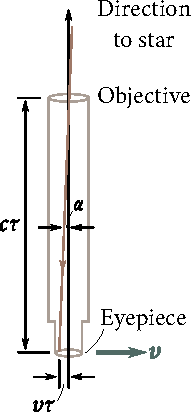
\includegraphics[scale=1]{figures/ch_21/fig_21_1.pdf}
		% \caption[]{}
        \caption[]{Đề án thí nghiệm của Bradley để xác định tốc độ ánh sáng. Hướng tới một ngôi sao nhìn trong kính thiên văn là vuông góc với mặt phẳng quỹ đạo của trái đất. Góc giữa hướng tới ngôi sao và vector vận tốc trái đất $v$ sẽ là $\pi/2$ trong cả năm.}
		\label{fig:21_1}
	\end{center}
	\vspace{-0.8cm}
\end{figure}

Do đó, vị trí nhìn thấy của một ngôi sao di chuyển tương đối với vị trí thật của nó một góc $\alpha$.
Vector vận tốc của trái đất quay liên tục trong mặt phẳng quỹ đạo.
Do đó, trục kính thiên văn cũng quay, tạo thành một hình nón hướng về phía ngôi sao.
Theo đó, vị trí nhìn thấy của ngôi sao trên thiên cầu tạo thành một hình tròn mà đường kính góc của nó là $2\alpha$.
Nếu hướng về phía ngôi sao tạo một góc khác góc vuông với mặt phẳng quỹ đạo trái đất, vị trí nhìn thấy của ngôi sao tạo thành một elip với trục chính có kích thước góc $2\alpha$.
Với một ngôi sao trong mặt phẳng quỹ đạo, elip suy biến thành đường thẳng.

Bradley tìm thấy từ quan sát thiên văn rằng  $2\alpha=\ang{;40.9;}$.
Giá trị tương ứng của $c$ nhận được từ \eqn{21_1} is \SI{303000}{km.s^{-1}}.

Ở điều kiện mặt đất, tốc độ ánh sáng được đo lần đầu tiên bởi nhà khoa học Pháp Armand Fizeau (1819-1896) vào năm 1849.
Bố cục thí nghiệm của ông như trong \fig{21_2}.
Ánh sáng từ nguồn S chiếu lên gương bán mạ.
Ánh sáng phản xạ từ gương đi tới cạnh của đĩa răng quay nhanh.
Mỗi khi không gian giữa các răng đối diện với tia sáng, một xung ánh sáng được tạo ra đi tới gương M và phản xạ trở lại.
Nếu tại thời điểm tia sáng trở lại đĩa mà không gian giữa các răng đối diện với tia sáng, xung phản xạ một phần đi xuyên qua gương bán mạ và đi tới mắt người quan sát.
Nếu một răng của đĩa ngáng đường xung phản xạ, người quan sát không thấy ánh sáng.

\begin{figure}[!htb]
	\begin{center}
		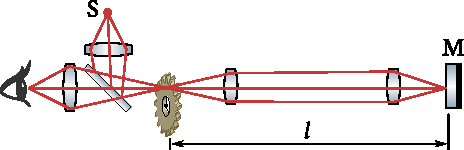
\includegraphics[scale=1]{figures/ch_21/fig_21_2.pdf}
		% \caption[]{}
        \caption[]{Thiết lập thí nghiệm của Fizeau để đo tốc độ ánh sáng. Ánh sáng từ nguồn S chiếu lên gương bán mạ.
		Ánh sáng phản xạ từ gương đi tới cạnh của đĩa răng quay nhanh. Mỗi khi không gian giữa các răng đối diện với tia sáng, một xung ánh sáng được tạo ra đi tới gương M và phản xạ trở lại. Nếu tại thời điểm tia sáng trở lại đĩa mà không gian giữa các răng đối diện với tia sáng, xung phản xạ một phần đi xuyên qua gương bán mạ và đi tới mắt người quan sát.
		Nếu một răng của đĩa ngáng đường xung phản xạ, người quan sát không thấy ánh sáng.}
		\label{fig:21_2}
	\end{center}
	\vspace{-0.8cm}
\end{figure}

Trong khoảng thời gian $\tau=2l/c$ cần thiết để ánh sáng đi hết quãng đường tới gương M và trở lại, đĩa quay một góc $\Delta{\omega}=\omega\tau=2l\omega/c$, với $\omega$ là vận tóc góc của đĩa.
Giả sử số lượng răng đĩa là $N$.
Do đó, góc ở tâm của hai răng kề là $\alpha = 2\pi/N$.
Ánh sáng không trở lại mắt người quan sát với vận tốc đĩa mà trong thời gian $\tau$ quay một góc $\alpha/2, 3\alpha/2, \ldots, (m-1/2)\alpha$, vân vân.
Do đó, điều kiện không thấy ánh sáng thứ $m$ có dạng
\begin{equation*}
	\Delta{\omega} = \parenthesis{m - \frac{1}{2}} \alpha \quad \text{or} \quad \frac{2l\omega}{c} = \parenthesis{m - \frac{1}{2}} \frac{2\pi}{N}.
\end{equation*}

\noindent
Theo công thức này, biết $l$, $N$, và vận tốc góc $\omega_m$ khi có chặn ánh sáng thứ $m$, ta có thể tìm được $c$.
Trong thí nghiệm của Fizeau, $l$ khoảng \SI{8.6}{km}.
Giá trị \SI{313000}{km.s^{-1}} được nhận cho $c$.

Vào  1928, tế bào Kerr (xem \sect{19_7}) được sử dụng để đo tốc độ ánh sáng.
Họ có thể làm gián đoạn tia sáng với tần số cao hơn nhiều (khoảng \SI{e7}{s^{-1}}) so với khi sử dụng đĩa răng quay.
Điều này làm cho các phép đo $c$ khả thi với $l$ ở bậc vài mét.

Albert Michelson thực hiện một vài phép đo tốc độ ánh sáng sử dụng phương pháp quay lăng kính.
Trong thí nghiệm của Michelson thực hiện vào năm 1932, ánh sáng được truyền trong ống dài \SI{1.6}{km} mà không khí được rút ra.

Hiện nay, tốc độ ánh sáng trong chân không được lấy bằng với    
\begin{equation}\label{eq:21_2}
	c = 299792.5 \pm \SI{0.1}{km.s^{-1}}.
\end{equation}

\noindent
Ta phải chú ý rằng trong tất cả thí nghiệm mà ánh sáng bị gián đoạn, vận tốc nhóm của sóng ánh sáng được xác định, không phải vận tốc pha.
Trong không khí, hai vận tốc này hầu như trùng nhau.

\section{Thí nghiệm của Fizeau}\label{sec:21_2}

Tới hiện tại, ta cho rằng các nguồn, máy thu, và các vật thể khác liên quan tới sự truyền ánh sáng là tĩnh.
Nó là tự nhiên khi quan tâm tới chuyển động của nguồn sáng ảnh hưởng tới sự truyền ánh sáng như thế nào.
Ở đây, nó trở nên cần thiết để đề cập tới những gì chuyển động diễn ra.
Ta thiết lập trong \sect{14_11} rằng chuyển động của nguồn hoặc máy thu của sóng âm đối với môi trường mà những sóng này truyền qua ảnh hưởng tới quá trình diễn ra hiện tương âm thanh (hiệu ứng Doppler ), và, kết quả là, có thể xác định.

Lý thuyết sóng bắt đầu đối xử với ánh angs như sóng đàn hồi truyền trong một môi trường giả thuyết gọi là ether.
Sau khi Maxwell cải tiến lý thuyết của ông ấy, ether được thay thế bằng một ether mang sóng và trường điện từ.
Ether này là một loại môi trường lấp đầy đặc biệt, giống như tiền thân ether đàn hồi của nó, nó truyền qua mọi vật thể trong toàn bộ vũ trụ.
Vì ether là một môi trường nhất định, có thể dựa vào việc xác định chuyển động của các vật thể, ví dụ nguồn sáng hoặc máy thu, đối với môi trường này.
Đặc biệt, sự tồn tại của một ``sóng ether'' thổi quanh trái đất trong chuyển động của nó về mặt trời nên được mong đợi.

Nguyên lý tương đối của Galileo được thiết lập trong cơ học.
Theo nó, mọi hệ quy chiếu quán tính là tương đương trong cơ học.
Việc phát hiện ether sẽ giúp có thể tách (với sự giúp đỡ của hiện tượng quang học) một hệ quy chiếu tuyệt đối, chiếm ưu thế đặc biệt ( liên quan tới ether).
Do đó, chuyển động của các hệ quy chiếu khác được xem xét đối với hệ quy chiếu tuyệt đối này.

Do đó, việc thiết lập cách ether tương tác với vật thể chuyển động, là một vấn đề nguyên lý.
Có ba cách có thể xem xét: (1) ether hoàn toàn không bị xáo trộn bởi vật thể chuyển động, (2) ether được mang theo một phần bởi các vật thể chuyển động, nhận được vận tốc $\alpha v$, với $v$ là vận tốc của một vật thể đối với hệ quy chiếu tuyệt đối, và $\alpha$ là hệ số kéo theo nhỏ hơn một đơn vị, và (3) ether được mang theo toàn bộ với vật thể chuyển động, ví dụ bởi trái đất, giống như cách mà vật thể trong chuyển động của nó mang theo các lớp khí liền kề bề mặt của nó.
Tuy nhiên, khả năng cuối cùng bị bác bỏ bởi sự tồn tại của hiện tượng quang sai.
Ta đã thiết lập trong phần trước rằng sự thay đổi vị trí nhìn thấy của các ngôi sao có thể giải thích bởi chuyển động của kính thiên văn đối với hệ quy chiếu (môi trường) mà sóng ánh sáng được truyền.

Để xác định liệu ether có được mang theo bởi vật thể chuyển động, Fizeau thực hiện thí nghiệm sau vào năm 1851.
Một chùm tia sáng song song từ nguồn S được chia bởi bản bán mạ P thành hai tia $1$ và $2$ (\fig{21_3}).
Như là kết quả của sự phản xạ trên gương M$_1$, M$_2$ và M$_3$, các tia sáng, sau khi đi qua quãng đường bằng nhau $L$, một lần nữa tới bản P.
Tia $1$ một phần đi qua P, trong khi tia $2$ một phần phản xạ.
Kết quả là, hai tia kết hợp $1'$ và $2'$ được tạo ra.
Chúng tạo ra một hình ảnh giao thoa ở dạng vân trong mặt phẳng tiêu cự của một kính thiên văn.
Hai ống dọc theo đó nước có thể đi qua với vận tốc $u$ theo hướng chỉ bởi mũi tên được đặt trên đường đi của các chùm tia $1$ và $2$.
Tia $2$ truyền qua cả hai ống ngược chiều với dòng chảy của nước, và tia $1$ theo dòng chảy.

\begin{figure}[!htb]
	\begin{center}
		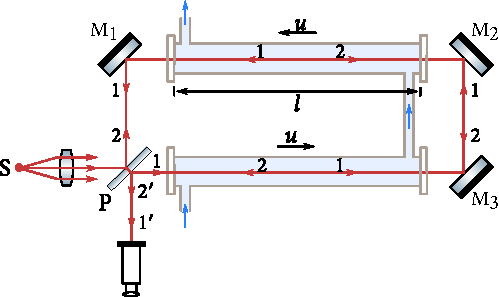
\includegraphics[scale=1]{figures/ch_21/fig_21_3.pdf}
		% \caption[]{}
        \caption[]{Thí nhiệm giao thoa kế của Fizeau để xác định vai trò của ether trong vật thể chuyển động. Một chùm sáng song song từ nguồn S được chia bởi bản bán mạ P thành hai chùm $1$ và $2$.}
		\label{fig:21_3}
	\end{center}
	\vspace{-0.8cm}
\end{figure}

Khi nước tĩnh, chùm $1$ và $2$ đi quãng đường $L$ trong cùng khoảng thời gian.
Nếu nước chuyển động một phần mang theo ether, thì khi dòng nước chảy, tia $2$ truyền ngược dòng nước, sẽ tốn nhiều thời gian hơn để đi hết quãng đường $L$ hơn tia $1$ di theo hướng dòng chảy.
Kết quả là, có một hiệu đường đi giữa hai tia, và hình ảnh giao thoa sẽ xuất hiện.

Hiệu đường đi mà ta quan tâm chỉ xuất hiện trong đường đi của tia sáng trong nước.
Quãng đường này dài $2l$.
Đặt vận tốc ánh sáng trong nước đối với ether là $v$.
Khi ether không được mang theo bởi nước, tốc độ ánh sáng đối với bố trí sẽ trùng với $v$.
Giả sử nước trong chuyển động của nó một phần mang theo ether, truyền cho ether vận tốc $\alpha u$ đối với bố trí ($u$ là vận tốc của nước, và $\alpha$ là hệ số kéo theo).
Do đó, vận tốc của ánh sáng đối với bố trí sẽ là $v+\alpha u$ cho tia $1$ và $v-\alpha u$ cho tia $2$.
Tia $1$ đi hết quãng đường $2l$ trong thời gian $t_1=2l/(v+\alpha u)$, và $2$ trong thời gian $t_2=2l/(v-\alpha u)$.
Có thể thấy từ \eqn{16_54} rằng quang trình để đi hết trong thời gian $t$ là $ct$.
Do đó, hiệu đường đi của các tia $1$ và $2$ là $\delta=c(t_2-t_1)$.
Chia $\delta$ với $\lambda_0$, ta được số vân của hệ giao thoa dịch chuyển khi dòng nước chảy:
\begin{equation*}
	\Delta{N} = \frac{c(t_2-t_1)}{\lambda_0} = \frac{c}{\lambda_0} \parenthesis{\frac{2l}{v-\alpha u} - \frac{2l}{v+\alpha u}} = \frac{4cl\alpha u}{\lambda_0 (v^2 - \alpha^2 u^2)}.
\end{equation*}

Fizeau khám phá ra rằng vân giao thoa đúng là bị dịch chuyển.
Giá trị của hệ số kéo theo liên quan tới độ dịch chuyển này là
\begin{equation}\label{eq:21_3}
	\alpha = 1 - \frac{1}{n^2},
\end{equation}

\noindent
với $n$ là chiết suất của nước.
Do đó, thí nghiệm của Fizeau chỉ ra rằng ether (nếu nó tồn tại) được mang theo bởi nước chuyển động chỉ một phần.

Có thể dễ dàng thấy rằng kết quả thí nghiệm của Fizeau được giải thích bằng định luật cộng vận tốc tương đối tính.
Theo phần đầu của phương trình (8.27) trong chương I, vận tốc $v_x$ và $v_x'$ của một vật thể trong hệ quy chiếu K và K$'$ được liên hệ bởi biểu thức
\begin{equation}\label{eq:21_4}
	v_x = \frac{v_x' + v_0}{1 + v_0 v_x'/c^2}
\end{equation}

\noindent
($v_0$ là vận tốc hệ quy chiếu K$'$ đối với hệ quy chiếu K).

Ta hãy liên hệ hệ quy chiếu K với bố trí của Fizeau, và hệ quy chiếu K$'$ với nước chảy.
Bây giờ, $v_0$ sẽ được thay bằng vận tốc của nước $u$, $v_x'$ thay bằng vận tốc ánh sáng đối với nước $c/n$, cuối cùng, $v_x$ được thay bằng vận tốc ánh sáng đối với dụng cụ $\ab{v}{inst}$.
Đưa các giá trị này vào \eqn{21_4} dẫn đến
\begin{equation*}
	\ab{v}{inst} = \frac{c/n + u}{1 + u(c/n)c^2} = \frac{(c/n) + u}{1 + u/(cn)}.
\end{equation*}

\noindent
Vận tốc của nước $u$ nhỏ hơn rất nhiều so với $c$.
Biểu thức nhận được do đó có thể đơn giản hóa như sau:
\begin{equation}\label{eq:21_5}
	\ab{v}{inst} = \frac{(c/n) + u}{1 + u/(cn)} = \approx \parenthesis{\frac{c}{n}+u} \parenthesis{1 - \frac{u}{cn}} \approx \frac{c}{n} + u \parenthesis{1 - \frac{1}{n^2}}
\end{equation}

\noindent
[Ta đã bỏ qua số hạng $u^2/(cn)$].

Theo khái niệm cổ điển, vận tốc ánh sáng đối với dụng cụ $\ab{v}{inst}$ bằng tổng của vận tốc ánh sáng đối với ether, tức là, $c/n$, và vận tốc của ether đối với dụng cụ, tức là, $\alpha u$:
\begin{equation*}
	\ab{v}{inst} = \frac{c}{n} + \alpha u.
\end{equation*}

\noindent
So sánh với \eqn{21_5} cho giá trị nhận được bởi Fizeau cho hệ số kéo theo $\alpha$ [xem \eqn{21_3}].

Nên nhớ rằng chỉ có vận tốc ánh sáng trong chân không là bằng nhau trong mọi hệ quy chiếu.
Vận tốc của nó trong vật chất khác nhau trong các hệ quy chiếu khác nhau.
Nó có giá trị $c/n$ trong hệ quy chiếu gắn với môi trường mà ánh sáng truyền qua.

\section{Thí nghiệm của Michelson}\label{sec:21_3}

Vào năm 1881, Michelson thực hiện thí nghiệm nổi tiếng mà ông ấy nỗ lực xác định chuyển động của trái đất đối với ether (gió ether).
Vào năm 1887, ông thực hiện lại thí nghiệm của ông ấy với Morley trên một dụng cụ đã cải tiến.
Thí nghiệm sử dụng bởi Michelson và Morley được chỉ ra trong \fig{21_4}.
Một nền gạch nâng một máng hình khuyên bằng sắt chứa thủy ngân.
Một cái phao gỗ có hình dạng của nửa dưới của một chiếc bánh donut cắt ngang nổi trên thủy ngân.
Chiếc phao nâng một phiến đá hình vuông lớn.
Thiết kế này cho phép xoay phiến đá quanh trục thẳng đứng của hệ một cách trơn tru.
Giao thoa kế Michelson (xem \fig{17_6}) được lắp đặt lên phiến đá.
Giao thoa kế được điều chỉnh sao cho cả hai tia trước khi trở về gương bán mạ đi qua một đoạn trùng với đường chéo của phiến đá vài lần.
Một sơ đồ của đường truyền tia sáng được chỉ ra trong \fig{21_5}.
Ký hiệu trong hình này tương ứng được sử dụng trong \fig{17_16}.

\begin{figure}[!htb]
	\begin{center}
		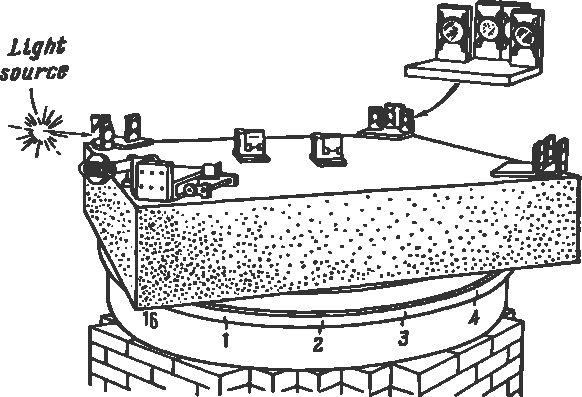
\includegraphics[scale=1]{figures/ch_21/fig_21_4.pdf}
		% \caption[]{}
        \caption[]{Thí nghiệm Michelson và Morley. Một nền gạch nâng một máng hình khuyên bằng sắt chứa thủy ngân. Một cái phao gỗ có hình dạng của nửa dưới của một chiếc bánh donut cắt ngang nổi trên thủy ngân. Chiếc phao nâng một phiến đá hình vuông lớn. Thiết kế này cho phép xoay phiến đá quanh trục thẳng đứng của hệ một cách trơn tru.}
		\label{fig:21_4}
	\end{center}
	\vspace{-0.8cm}
\end{figure}

\begin{figure}[!htb]
	\begin{center}
		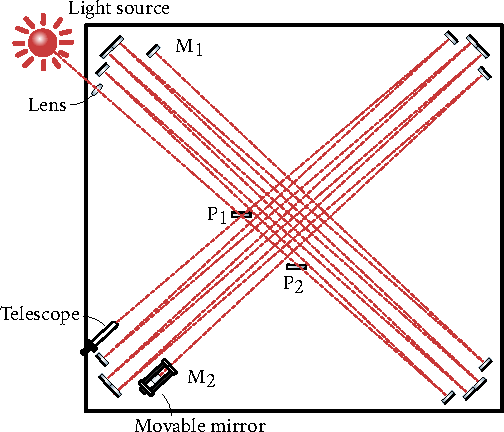
\includegraphics[scale=1]{figures/ch_21/fig_21_5.pdf}
		% \caption[]{}
        \caption[]{Điều chỉnh giao thoa kế Michelson. Giao thoa kế được điều chỉnh sao cho cả hai tia trước khi trở về gương bán mạ đi qua một đoạn trùng với đường chéo của phiến đá vài lần. Ký hiệu trong hình này tương ứng được sử dụng trong \fig{17_16}.}
		\label{fig:21_5}
	\end{center}
	\vspace{-0.8cm}
\end{figure}

Thí nghiệm được dựa trên lý do sau. Giả sử trục  PM$_2$ (\fig{21_6}) trùng với hướng chuyển động của Trái đất đối với ether.
Kết quả là, thời gian cần thiết để tia $1$ đi hết quãng đường tới gương M$_1$ và trở về sẽ khác với thời gian cần thiết để tia $2$ đi hết quãng đường PM$_2$P.
vậy thì, thậm chí khi chiều dài của cả hai trục là bằng nhau, tia $1$ và $2$ sẽ có một hiệu đường đi nhất định.
Nếu ta quay bố cục một góc \ang{90}, các trục sẽ thay đổi vị trí, và hiệu quãng đường sẽ thay đổi dấu.
Điều này sẽ biểu hiện ở độ dịch chuyển vân giao thoa mà độ lớn, đã được chỉ ra bởi tính toán của Michelson, có thể được xác định dễ dàng.

\begin{figure}[!htb]
	\begin{minipage}[t]{0.6\linewidth}
		\begin{center}
			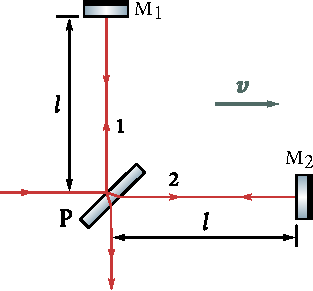
\includegraphics[scale=1]{figures/ch_21/fig_21_6.pdf}
			% \caption[]{}
            \caption[]{Lý luận của thí nghiệm Michelson và Morley, cho rằng trục giao thoa kế PM$_2$ trùng với hướng chuyển động của Trái đất đối với ether. Thì, thời gian cần thiết để tia $1$ đi hết quãng đường tới M$_1$ và trở về sẽ khác với thời gian cần thiết để tia $2$ đi hết quãng đường PM$_2$P. Kết quả là, thậm chí là khi độ dài hai trục bằng nhau, tia $1$ và $2$ sẽ nhận một hiệu đường đi nhất định.
			Quay bố trí một góc \ang{90}, các trục sẽ thay đổi vị trí, và hiệu đường đi sẽ đổi dấu của nó.}
			\label{fig:21_6}
		\end{center}
	\end{minipage}
	\hfill{ }%space{-0.05cm}
	\begin{minipage}[t]{0.36\linewidth}
		\begin{center}
			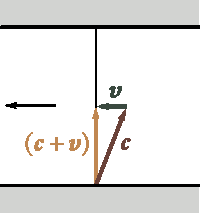
\includegraphics[scale=1]{figures/ch_21/fig_21_7.pdf}
            % \caption[]{}
			\caption[]{Xem xét để tính thời gian $t_1$. Giả sử rằng có một vụ phóng có vận tốc $c$ đối với nước phải băng qua một con sông với vận tốc dòng chảy $v$ theo hướng vuông góc với bờ. Để vụ phóng đi theo hướng cần thiết, vận tốc của nó $c$ với nước phải hướng như đã chỉ ra.}
			\label{fig:21_7}
		\end{center}
	\end{minipage}
\vspace{-0.4cm}
\end{figure}

Để tính độ dịch chuyển của vân giao thoa, ta hãy tìm thời gian cần thiết bởi tia $1$ và $2$ để đi hết các quãng đường liên quan.
Cho rằng vận tốc trái đất đối với ether là $v$.
Nếu ether không được mang theo bởi trái đất và vận tốc ánh sáng đối với ether là $c$ (chiết suất của không khí gần như bằng một), thì vận tốc ánh sáng đối với thiết bị sẽ là $c - v$ theo hướng PM$_2$ và $c + v$ theo hướng M$_2$P.
Do đó, thời gian cần thiết cho $2$ được xác định bởi công thức
\begin{equation}\label{eq:21_6}
	t_2 = \frac{l}{c-v} + \frac{l}{c+v} = \frac{2lc}{c^2-v^2} = \frac{2l}{c} \frac{1}{(1-v^2/c^2)} \approx \frac{2l}{c} \parenthesis{1 + \frac{v^2}{c^2}}
\end{equation}

\noindent
(vận tốc Trái đất trên quỹ đạo của nó là \SI{30}{km.s^{-1}}, do đó, $v^2/c^2= \num{e-8}\ll 1$).

Trước khi bắt đầu tính thời gian $t_1$, ta hãy xem xét ví dụ sau từ cơ học.
Giả sử rằng một vụ phóng có vận tốc $c$ đối với nước phải băng qua một con sông với vận tốc dòng chảy $v$ theo hướng vuông góc với bờ (\fig{21_7}).
Để vụ phóng đi theo hướng cần thiết, vận tốc của nó $c$ với nước phải phải hướng như hình.
Do đó, vận tốc của vụ phóng với bờ sẽ là $|c+v|=\sqrt{c^2-v^2}$.
Vận tốc tia $1$ đối với bố trí (theo như Michelson) sẽ như nhau.
Kết quả là, thời gian cần thiết cho tia 1 là\footnote{Ta đã sử dụng công thức $\sqrt{1- x}\approx 1-x/2$ và $1/(1-x) \approx 1+x$, cho giá trị $x$ nhỏ.}
\begin{equation}\label{eq:21_7}
	t_1 = \frac{2l}{\sqrt{c^2-v^2}} = \frac{2l}{c} \frac{1}{\sqrt{1-v^2/c^2}} \approx \frac{2l}{c} \parenthesis{1 + \frac{1}{2} \frac{v^2}{c^2}}.
\end{equation}

Thay $t_2$ và $t_1$ trong biểu thức $\Delta=c(t_2 - t_1)$ giá trị của chúng từ biểu thức \eqref{eq:21_6} và \eqref{eq:21_7}, ta có hiệu đường đi của tia $1$ và $2$:
\begin{equation*}
	\Delta = 2l \bracket{\parenthesis{1+\frac{v^2}{c^2}} - \parenthesis{1 + \frac{1}{2} \frac{v^2}{c^2}}} = l \frac{v^2}{c^2}.
\end{equation*}

\noindent
Khi hệ thống quay một góc \ang{90}, hiệu đường đi đổi dấu.
Kết quả là, số vân hệ giao thoa bị dịch chuyển là
\begin{equation}\label{eq:21_8}
	\Delta{N} = \frac{2\Delta}{\lambda_0} = 2 \frac{l}{\lambda_0} \frac{v^2}{c}.
\end{equation}

Độ dài trục $l$ (tính đến phản xạ nhiều mặt) là \SI{11}{m}.
Bước sóng ánh sáng sử dụng bởi Michelson và Morley là \SI{0.59}{\micro\metre}.
Sử dụng những giá trị này vào \eqn{21_8} cho
\begin{equation*}
	\Delta{N} = \frac{2\times 11}{\num{0.59e-6}} \times \num{e-8} = 0.37 \approx 0.4\text{ vân}.
\end{equation*}

\noindent
Có thể xác định độ dịch chuyển bậc của $0.01$ vân nhờ bố trí.
Nhưng không có sự dịch chuyển nào của vân giao thoa được xác định.
Thí nghiệm được lặp lại nhiều lần vào những thời điểm khác nhau trong ngày để loại trừ khả năng mặt phẳng ngang vuông góc với vector vận tốc quỹ đạo của Trái đất tại thời điểm đo.
Kết quả là, thí nghiệm được lặp lại nhiều lần trong các mùa khác nhau trong năm (trong một năm, vector vận tốc quỹ đạo của trái đất quay trong không gian góc \ang{360}), và liên tục nhận được kết quả phủ định.
Nỗ lực xác định gió ether không thành công, ether vẫn chưa thể xác định.

Một vài nỗ lực được thực hiện để giải thích kết quả phủ định của thí nghiệm Michelson mà không bác bỏ giả thuyết sự tồn lại của ether.
Nhưng tất cả những nỗ lực này là vô căn cứ.
Một giải thích toàn diện không mâu thuẫn của tất cả sự thật thực nghiệm bao gồm kết quả thí nghiệm của Michelson được đưa ra bởi Albert Einstein vào năm 1905.
Ông ấy kết luận rằng ether, tức là, một môi trường đặc biệt mà có thể sử dụng như một hệ quy chiếu tuyệt đối, không tồn tại.
Theo đó, Einstein mở rộng nguyên lý cơ học tương đối tính cho mọi hiện tượng vật lý không có ngoại lệ nào.
Ông tiên đề hóa phù hợp với số liệu thực nghiệm rằng tốc độ ánh sáng trong chân không là như nhau trong mọi hệ quy chiếu quán tính và không phụ thuộc vào chuyển động của nguồn sáng và nguồn thu.

Nguyên lý tương đối và nguyên lý hằng số tốc độ ánh sáng tạo thành cơ sở của thuyết tương đối hẹp phát triển bởi Einstein (xem Chương 8 của tập I).

\section{Hiệu ứng Doppler}\label{sec:21_4}

Trong sóng âm, sự thay đổi tần số do hiệu ứng Doppler được xác định bởi vận tốc của nguồn âm và máy thu đối với môi trường truyền sóng âm [xem \eqn{14_78}].
Hiệu ứng Doppler cũng tồn tại đối với sóng ánh sáng.
Nhưng không có môi trường đặc biệt nào đóng vai trò như môi trường truyền tróng điện từ.
Do đó, dịch chuyển Doppler của tần số sóng ánh sáng được xác định chỉ bởi vận tốc tương đối của nguồn phát và máy thu.

Ta hãy gắn gốc tọa độ của hệ quy chiếu K với một nguồn sáng và gốc tọa độ của hệ quy chiếu K$'$ với một máy thu (\fig{21_8}).
Ta sẽ định hướng trục $x$ và $x'$, như bình thường thường, theo vector vận tốc $v$ mà hệ quy chiếu K$'$ (tức là, máy thu) di chuyển tương đối với hệ quy chiếu K (tức là, nguồn).
Phương trình của một sóng ánh sáng phẳng phát ra từ nguồn theo hướng của máy thu sẽ có dạng sau trong hệ quy chiếu K:
\begin{equation}\label{eq:21_9}
	E(x,t) = A \cos\bracket{\omega \parenthesis{t - \frac{x}{c}} + \alpha}.
\end{equation}

\noindent
Ở đây, $\omega$ là tần số góc của sóng trong hệ quy chiếu gắn với nguồn, tức là, tần số dao động của nguồn.
Ta giả thuyết rằng sóng ánh sáng truyền trong chân không; do đó, vận tốc pha là $c$.

\begin{figure}[!htb]
	\begin{center}
		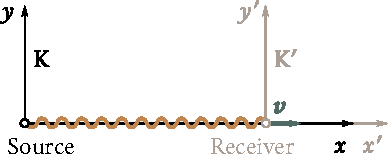
\includegraphics[scale=1]{figures/ch_21/fig_21_8.pdf}
		% \caption[]{}
        \caption[]{Hiệu ứng Doppler cho sóng ánh sáng. Ta hãy gắn gốc tọa độ của hệ quy chiếu K với nguồn sáng và gốc tọa độ của hệ quy chiếu K$'$ với máy thu. Định hướng trục $x$ và $x'$, theo vector vận tốc $v$ mà hệ quy chiếu K$'$ (máy thu) chuyển động tương đối với hệ quy chiếu K (nguồn).}
		\label{fig:21_8}
	\end{center}
	\vspace{-0.8cm}
\end{figure}

Theo thuyết tương đối, các quy luật tự nhiên có cùng dạng trong mọi hệ quy chiếu quán tính.
Do đó, trong hệ quy chiếu K$'$, sóng cho bởi \eqn{21_9} sẽ được mô tả bởi phương trình
\begin{equation}\label{eq:21_10}
	E(x',t') = A' \cos\bracket{\omega' \parenthesis{t' - \frac{x'}{c}} + \alpha'},
\end{equation}

\noindent
với $\omega'$ là tần số góc trong hệ quy chiếu K$'$, tức là, tần số nhận được bởi máy thu.
Ta đã cung cấp mọi đại lượng ngoại trừ $c$, thứ bất biến trong mọi hệ quy chiếu, với dấu phẩy.

Ta có thể nhận phương trình của sóng trong hệ quy chiếu K$'$ từ một phương trình trong hệ quy chiếu K bằng cách thay $x$ và $t$ thành $x'$ và $t'$ với sự giúp đỡ của phép biến đổi Lorentz.
Đưa vào thay cho $x$ và $t$ trong \eqn{21_9} các giá trị phù hợp với phương trình (8.17) của tập I, ta có
\begin{equation*}
	E(x',t') = A\cos\bracket{\omega \parenthesis{ \frac{t'+(v/c^2)x'}{\sqrt{1-v^2/c^2}} - \frac{x'+vt'}{c \sqrt{1-v^2/c^2}} } +\alpha }
\end{equation*}

\noindent
(phần $v_0$ được thay bởi $v$).
Phương trình sau dễ dàng được biến đổi thành phương trình sau:
\begin{equation}\label{eq:21_11}
	E(x',t') = A\cos\bracket{\omega \parenthesis{ \frac{1-v/c}{\sqrt{1-v^2/c^2}} } \parenthesis{t' - \frac{x'}{c}} +\alpha }.
\end{equation}

Phương trình \eqref{eq:21_11} miêu tả cùng một sóng trong hệ quy chiếu K$'$ như \eqn{21_10}.
Do đó, phải có liên hệ sau
\begin{equation*}
	\omega' = \omega \frac{1-v/c}{\sqrt{1-v^2/c^2}} = \omega \parenthesis{\frac{1-v/c}{1+v/c}}^{1/2}.
\end{equation*}

\noindent
Ta hãy thay đổi kí hiệu: ta sẽ gọi tần số $\omega$ của nguồn là $\omega_0$, và tần số $\omega'$ của máy thu bằng $\omega$.
Phương trình trước đó do đó trở thành
\begin{equation}\label{eq:21_12}
	\omega = \omega_0 \parenthesis{\frac{1-v/c}{1+v/c}}^{1/2}.
\end{equation}

\noindent
Thay đổi từ tần số góc thành tần số thông thường, ta có
\begin{equation}\label{eq:21_13}
	\nu = \nu_0 \parenthesis{\frac{1-v/c}{1+v/c}}^{1/2}.
\end{equation}

Vận tốc $v$ của máy thu đối với nguồn trong \eqns{21_12}{21_13} là một đại lượng đại số.
Khi máy thu chuyển động ra xa nguồn, $v > 0$, và theo \eqn{21_12}, $\omega<\omega_0$; khi máy thu tới gần nguồn, $v<0$, do đó $\omega>\omega_0$.
Khi $v\ll c$, \eqn{21_12} có thể được viết xấp xỉ như sau:
\begin{equation*}
	\omega \approx \omega_0 \bracket{ \frac{1 -(1/2)(v/c)}{1 + (1/2)(v/c)} } \approx \omega_0 \parenthesis{1 - \frac{1}{2} \frac{v}{c}} \parenthesis{1 - \frac{1}{2} \frac{v}{c}}.
\end{equation*}

\noindent
Do đó, sau khai triển Taylor gần $v=0$ và giới hạn bản thân tới số của bậc $v/c$, ta có
\begin{equation}\label{eq:21_14}
	\omega = \omega_0 \parenthesis{1 - \frac{v}{c}}.
\end{equation}

\noindent
Từ công thức này, ta có thể tìm độ thay đổi tương đối tần số:
\begin{equation}\label{eq:21_15}
	\frac{\Delta{\omega}}{\omega} = - \frac{v}{c}
\end{equation}

\noindent
($\Delta{\omega}$ là $\omega-\omega_o$).

Ta có thể chỉ ra rằng \textbf{hiệu ứng Doppler ngang} tồn tại cho sóng ánh sáng ngoài hiệu ứng dọc ta đã xem xét.
Nó bao gồm một sự giảm tần số nhận được bởi máy thu quan sát được khi vector vận tốc tương đối vuông góc với đường thẳng đi qua nguồn thu và máy phát\footnote{Chúng ta nhắc nhở độc giả rằng hiệu ứng Doppler ngang không tồn tại với sóng âm.} (khi, ví dụ, nguồn di chuyển theo một đường tròn mà tâm là máy thu).
Trong trường hợp này, tần số $\omega_0$ trong hệ quy chiếu của nguồn gắn với tần số $\omega$ trong hệ quy chiếu máy thu bởi liên hệ
\begin{equation}\label{eq:21_16}
	\omega = \omega_0 \parenthesis{1 - \frac{v^2}{c^2}}^{1/2} \approx \omega_0 \parenthesis{1 - \frac{1}{2} \frac{v^2}{c^2}}.
\end{equation}

Thay đổi tương đối trong tần số của hiệu ứng Doppler ngang
\begin{equation}\label{eq:21_17}
	\frac{\Delta{\omega}}{\omega} = - \frac{1}{2} \frac{v^2}{c^2},
\end{equation}

\noindent
tỷ lệ với bình phương của tỷ số $v/c$ và, kết quả là, nhỏ hơn đáng kể so với hiệu ứng dọc mà 
độ thay đổi tương đối trong tần số tỷ lệ thuận với bậc đầu tiên của $v/c$.

Sự tồn tại của hiệu ứng Doppler ngang được chứng minh thực nghiệm bởi nhà vật lý người Mỹ Herbert Ives (1882-1953) vào năm 1938.
Ông xác định độ thay đổi tần số của khí nguyên tử hydro trong tia dương cực (xem đoạn cuối của \sect{12_6}).

Vận tốc của nguyên tử cỡ \SI{2e8}{m.s^{-1}}.
Thí nghiệm này là xác nhận thực nghiệm trực tiếp sự chính xác của biến đổi Lorentz.

Trong trường hợp tổng quát, vector vận tốc tương đối có thể được phân tích thành hai thành phần một trong số đó hướng theo tia sáng, và phần còn lại vuông góc với nó.
Thành phần đầu tiên đóng góp vào hiệu ứng dọc, và thành phần thứ hai đóng góp vào hiệu ứng Doppler ngang.

Hiệu ứng Doppler dọc được sử dụng để xác định vận tốc bán kính của các ngôi sao.
Bằng cách đo độ chuyển vạch tương đối trong quang phổ của các ngôi sao, ta có thể sử dụng \eqn{21_12} để xác định $v$.

Chuyển động nhiệt của khối khí đang bức xạ, nhờ hiệu ứng Doppler, dẫn đến sự mở rộng vạch quang phổ.
Như một kết quả của chuyển động nhiệt hỗn loạn tự nhiên, mọi hướng của vận tốc nguyên tử đối với máy quang phổ là đồng xác xuất.
Do đó, bức xạ thu được dụng cụ bao gồm mọi tần số trong khoảng từ $\omega_0(1 - v/c)$ tới $\omega_o (1 + v/c)$, với $\omega_0$ là tần số phát ra bởi nguyên tử, và $v$ là vận tốc của chuyển động nhiệt [xem \eqn{21_14}].
Độ rộng của dãi quang phổ do đó là $2\omega_0v/c$.
Đại lượng
\begin{equation}\label{eq:21_18}
	\delta{\ab{\omega}{D}} = 2\omega_0 \frac{v}{c},
\end{equation}

\noindent
được gọi là \textbf{độ rộng Doppler của dãi quang phổ ($v$ là vận tốc có xác xuất lớn nhất của phân tử).
Độ lớn của mở rộng Doppler dãy quang phổ làm nó có thể đạt được vận tốc chuyển động nhiệt của phân tử và, kết quả là, nhiệt độ của khối khí đang bức xạ.
